% !TEX TS-program = xelatex 
%version 11/1/2019
\documentclass[14pt,a4paper]{extarticle}
\usepackage{fontspec}
\setmainfont{Nom Na Tong}
\usepackage{graphicx} 
\usepackage{pagecolor} 
\usepackage[%paperwidth=21cm,paperheight=100cm,
left=2cm,right=2cm,top=2cm,bottom=2cm,
]
{geometry} 
% \pagestyle{empty}



\usepackage{comment} 
\begin{document}
\parindent=0pt


\input{tdktoantap6jun26}




\def\úa{𦼇\ }
\def\hát{咭\ }
\def\măng{笀\ }
\def\ngơngác{魚\kern.125em 萼\kern.125em }
\def\heomay{囂 𩘄\ }
\def\côđơn{孤 單\ }
\def\langthang{郎 徜\ }
\def\thànhphố{城 舖\ }
\def\nhòa{𤍶\ }
\def\bàntay{盤 𢬣\ }
\def\Ngà{玡\ }
\def\phiến{片\ }
\def\lụa{縷\ }
\def\Xe{𦀺\ }
%\def\muốt{\raisebox{-.26ex}{\includegraphics[scale=.6]{muoost.pdf} }}

\def\nào{𱜢\kern.125em  }
\def\nay{𫢩\kern.125em } 
\def\HẠ{复\kern.125em }  %mùa hè
\def\ức{忆\kern.125em }
\def\đẫm{沉\kern.125em }
\def\dế{𧍝\kern.125em }
\def\ánh{映\kern.125em }
\def\tít{𨙌\kern.125em }
\def\tắp{潗\kern.125em }
\def\ảo{幻\kern.125em }
\def\ảnh{影\kern.125em }
\def \úp{挹\kern.125em }
\def\niệm{念\kern.125em }
\def\biển{汴\kern.125em }
\def\Phượng{楓 \kern.125em }
\def\nuối{𢗉 \kern.125em }
\def\VÀng{黄 \kern.125em }
\def\day{厓 \kern.125em }
\def\dứt{𠛣 \kern.125em }
\def\quay{乖 \kern.125em }
\def\phiêu{漂 \kern.125em }


\def\ơi{𠲖  \kern.125em }
\def\sàigòn{西 貢  \kern.125em }
\def\ngắn{𠦯 \kern.125em }
\def\diễm{艳 \kern.125em }
\def\sámhối{忏 悔 \kern.125em }
\def\Nhị{二\ }
\def\hỉ{喜 \kern.125em }
\def\lừng{㖫 \kern.125em }

\def\ngớt{𣲠 \kern.125em }
\def\toả{剉 \kern.125em }
\def\mân{𲠈\kern.125em }
\def\dựa{󰇰\kern.125em }
\def\sưởi{𤇧\kern.125em }
\def\heo{	囂\kern.125em }
\def\ngủ{𥄬\kern.125em }
\def\nếu{𠮩\kern.125em }
\def\bấn{絆\kern.125em }
\def\ảm{黯\kern.125em }

% bổ sung 

\def\úa{𦼇\ }
\def\hát{咭\ }
\def\măng{笀\ }
\def\heomay{囂 𩘄\ }
\def\côđơn{孤 單\ }
\def\langthang{郎 徜\ }
\def\thànhphố{城 舖\ }
\def\nhòa{𤍶\ }
\def\bàntay{盤 𢬣\ }
\def\Ngà{玡\ }
\def\phiến{片\ }
\def\lụa{縷\ }
\def\Xe{𦀺\ }
\def\ưu{憂\ }
\def\đốm{炶\ }
\def\nằng{能\ }
\def\imlìm{奄 𠿳\ }
\def\tịch{寂\ }
\def\nhanh{𨗜\ }
\def\ngủ{𥄬\ }
\def\thon{村\ }
\def\Nương{𢭗\ }
\def\Phố{舖\ }
\def\trau{捞\ }
\def\dỗi{𠾕\ }
\def\ANh{嬰\ }


\def\úa{𦼇\ }
\def\hát{咭\ }
\def\măng{笀\ }
\def\heomay{囂 𩘄\ }
\def\côđơn{孤 單\ }
\def\langthang{郎 徜\ }
\def\thànhphố{城 舖\ }
\def\nhòa{𤍶\ }
\def\bàntay{盤 𢬣\ }
\def\Ngà{玡\ }
\def\phiến{片\ }
\def\lụa{縷\ }
\def\Xe{𦀺\ }
\def\ưu{憂\ }
\def\đốm{炶\ }
\def\nằng{能\ }
\def\imlìm{奄 𠿳\ }
\def\tịch{寂\ }
\def\nhanh{𨗜\ }
\def\ngủ{𥄬\ }
\def\thon{村\ }
\def\Nương{𢭗\ }
\def\Phố{舖\ }



\def\tím{僣\ }
\def\dòng{𣳔\ }
\def\biền{便\ }
\def\bềnh{泙\ }
\def\biêng{梹\ }
\def\sim{枮\ }
\def\tuổithơ{\tuổi 𡮲\ }

\def\Chín{𤒙\ }


\def\úa{𦼇\ }
\def\hát{咭\ }
\def\măng{笀\ }
\def\heomay{囂 𩘄\ }
\def\côđơn{孤 單\ }
\def\langthang{郎 徜\ }
\def\thànhphố{城 舖\ }
\def\nhòa{𤍶\ }
\def\bàntay{盤 𢬣\ }
\def\Ngà{玡\ }
\def\phiến{片\ }
\def\lụa{縷\ }
\def\Xe{𦀺\ }
%\def\muốt{\raisebox{-.26ex}{\includegraphics[scale=.3]{muoost.pdf} }}
\def\muốt{\raisebox{-.3ex}{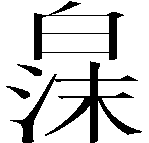
\includegraphics[scale=.5]{muốt.pdf} \kern-.1em}}


\def\bạt{跋}
\def\trán{顙}
\def\xứ{處}
\def\khô{枯}
\def\ngấn{痕}
\def\nua{孥}
\def\bé{𡭬}
\def\uẩn{酝}
\def\giùm{𡑓}
\def\rớm{滲}
\def\bương{𥮇}
\def\cấn{艮}
\def\sài{柴}
\def\lúa{穭}
\def\chậm{踸}
\def\sáo{筲}
\def\diều{鷂}
\def\khoắt{阔}
\def\Vương{𥿁}
\def\cánhđồng{\cánh 垌}
\def\XÁc{殻}
\def\VÀng{黄}
\def\thanhbình{清平}

\vspace*{.3\textheight}


%\begin{comment}



\pagecolor{magenta} \thispagestyle{empty}

{\setmainfont[Scale=4]{UTM HelvetIns} \color{yellow}TUYỂN TẬP THƠ CA}

\vspace*{3cm}


{\color{white}\begin{flushright}
{\small Chim ơi chết dưới cội hoa}

\chim \ơi \chết \dưới \cội \hoa

{\small Tiếng kêu rơi rụng giữa giang hà}

\tiếng \kêu \rơi \rụng \giữa \giang \hà

{\small Mai ta chết dưới cội đào }

\Mai \ta \chết \dưới \cội \đào

{\small Khóc ta xin nhỏ lệ vào thiên thu}

\khóc \ta \xin \Nhỏ \lệ \vào \THiên \thu
\end{flushright}}

\newpage 

\pagecolor{white}
\normalsize \thispagestyle{empty}

\vspace*{.25\textheight}

\begin{flushright}

Tháng sáu trời nắng tháng sáu trời mưa. 

Em giữ riêng em khoảng trời màu tím. 

Anh có trở về bước chân xin tìm đến. 

Có một khoảng trời tháng sáu của riêng anh.\bigskip 

{\color{magenta}\tháng\sáu\trời\nắng\tháng\sáu\trời\mưa

\em\giữ\riêng\em\khoảng\trời\màu\tím

\ANH\có\trở\về\bước\chân\xin\tìm\đến

\có\một\khoảng\trời\tháng\sáu\của\riêng\ANH}

\vfill 
\hrule \smallskip 

Chữ Nôm trong tuyển tập này sẽ viết thật to để dễ dàng nhận diện mặt chữ. Chữ Nôm của Nguyễn Du, Nguyễn Trãi, Hồ Xuân Hương và Nguyễn Đình Chiểu là chữ nôm  kinh điển. Chữ Nôm trong tuyển tập này là ngôn ngữ của thời đại.
%{\small Chim ơi chết dưới cội hoa}
%
%\chim \ơi \chết \dưới \cội \hoa
%
%{\small Tiếng kêu rơi rụng giữa giang hà}
%
%\tiếng \kêu \rơi \rụng \giữa \giang \hà
%
%{\small Mai ta chết dưới cội đào }
%
%\Mai \ta \chết \dưới \cội \đào
%
%{\small Khóc ta xin nhỏ lệ vào thiên thu}
%
%\khóc \ta \xin \Nhỏ \lệ \vào \THiên \thu
\end{flushright}

%\hrule

\newpage 




\small 

CHO EM và MÙA HẠ\\[1ex]
{\huge \cho \em \và \mùa \HẠ}\\[1ex]
\bigskip 


Hình như bên kia là mùa thu\\[1ex]
{\huge \hình \như \bên \kia \là \mùa \thu}\\[1ex]
Ngàn lá rụng mang theo lời tiễn biệt\\[1ex]
{\huge \ngàn \lá \rụng \mang \theo \Lời \tiễn \biệt}\\[1ex]
Nơi ký ức hoá vầng trăng đẫm ướt\\[1ex]
{\huge \nơi \ký \ức \hoá \vầng \trăng \đẫm \ướt}\\[1ex]
Con dế buồn rũ cỏ hát tình ca\\[1ex]
{\huge \con \dế \buồn \rũ \cỏ \hát \tình \ca}\\[1ex]
Bên kia là năm tháng đi qua\\[1ex]
{\huge \bên \kia \là \năm \tháng \đi \qua}\\[1ex]
Còn gặp lại cũng vô tình ánh mắt\\[1ex]
{\huge \còn \gặp \lại \cũng \vô \tình \ánh \mắt}\\[1ex]
Bông hồng ấy cuối chân trời tít tắp\\[1ex]
{\huge \bông \hồng \ấy \cuối \chân \trời \tít \tắp}\\[1ex]
Dẫu muộn phiền từng cánh mỏng manh rơi\\[1ex]
{\huge \dẫu \muộn \phiền \từng \cánh \mỏng \manh \rơi}\\[1ex]
Bên kia là còn lại mình tôi\\[1ex]
{\huge \bên \kia \là \còn \lại \mình \tôi}\\[1ex]
Mùa hạ và em xa vời ảo ảnh\\[1ex]
{\huge \mùa \HẠ \và \em \xa \vời \ảo \ảnh}\\[1ex]
Hoa cúc cháy trong nỗi niềm đa cảm\\[1ex]
{\huge \hoa \cúc \cháy \trong \nỗi \niềm \đa \cảm}\\[1ex]

\newpage 
Thuở yêu em trong trắng vô ngần\\[1ex]
{\huge \thuở \yêu \em \Trong \trắng \vô \ngần}\\[1ex]
Bên kia là còn lại dòng sông\\[1ex]
{\huge \bên \kia \là \còn \lại \dòng \sông}\\[1ex]
Cánh buồm anh nửa đời đi không hết\\[1ex]
{\huge \cánh \buồm \ANH \nửa \đời \đi \không \hết}\\[1ex]
Em xa quá, mùa thu thì chẳng biết\\[1ex]
{\huge \em \xa \quá \mùa \thu \thì \chẳng \biết}\\[1ex]
Có người úp mặt khóc hoàng hôn\\[1ex]
{\huge \có \người \úp \mặt \khóc \HOÀng \Hôn}\\[1ex]
Lẽ nào em không nhớ, lẽ nào quên\\[1ex]
{\huge \lẽ \nào \em \không \nhớ \lẽ \nào \quên}\\[1ex]
Giọt nước mắt đã tan thành hoài niệm\\[1ex]
{\huge \giọt \nước \mắt \đã \tan \THành \hoài \niệm}\\[1ex]
Thành muối mặn thành vô tư sóng biển\\[1ex]
{\huge \THành \muối \mặn \thành \vô \tư \sóng \biển}\\[1ex]
Để vơi đầy cùng năm tháng vì nhau\\[1ex]
{\huge \để \vơi \đầy \Cùng \năm \tháng \vì \nhau}\\[1ex]
Bên kia là còn lại nỗi đau\\[1ex]
{\huge \bên \kia \là \còn \lại \nỗi \đau}\\[1ex]
Khao khát ấy của một trời hoa phượng\\[1ex]
{\huge \khao \khát \ấy \của \một \trời \hoa \Phượng}\\[1ex]
Lẽ nào em, lẽ nào tôi hoang tưởng\\[1ex]
{\huge \lẽ \nào \em \lẽ \nào \tôi \hoang \tưởng}\\[1ex]
Lá vàng thu tiếc nuối giữa tay người\\[1ex]
{\huge \lá \VÀng \thu \tiếc \nuối \giữa \tay \người}\\[1ex]

\newpage Bên kia là day dứt khôn nguôi\\[1ex]
{\huge \bên \kia \là \day \dứt \khôn \nguôi}\\[1ex]
Đồng vọng mãi lời chia tay thầm lặng\\[1ex]
{\huge 垌 \vọng \mãi \Lời \chia \tay \thầm \lặng}\\[1ex]
Phải mùa hạ dâng hết mình cho nắng\\[1ex]
{\huge \phải \mùa \HẠ \dâng \hết \mình \cho \nắng}\\[1ex]
Nên mùa thu chớm lạnh đã se lòng\\[1ex]
{\huge \nên \mùa \thu 拈 \lạnh \đã \se \lòng}\\[1ex] 
Thì đừng buồn bốn phía mưa giăng\\[1ex]
{\huge \thì \đừng \buồn \bốn 𪰂 \mưa \giăng}\\[1ex]
Bong bóng vỡ theo về nguồn cội\\[1ex]
{\huge 𤂧 \bóng \vỡ \theo \về \nguồn \cội}\\[1ex]
Ngắt cánh phù dung ngồi đếm tuổi\\[1ex]
{\huge \ngắt \cánh \phù \dung \ngồi 掂 \tuổi}\\[1ex]
Thấy trong hư vô khuôn mặt của mình\\[1ex]
{\huge \thấy \trong \hư \vô \khuôn \mặt \của \mình}\\[1ex]
Thì ta quay về tìm lại dòng sông\\[1ex]
{\huge \thì \ta \quay \về \tìm \lại \dòng \sông}\\[1ex]
Tìm lại xác thân phiêu bồng một thuở\\[1ex]
{\huge \tìm \lại \xác \thân \phiêu \bồng \một \thuở}\\[1ex]
Để thấp thoáng em hiện về đâu đó\\[1ex]
{\huge \để \thấp \thoáng \em \hiện \về \đâu \đó}\\[1ex]
Mùa hạ ấy xa như có thật trong đời.\\[1ex]
{\huge \mùa \HẠ \ấy \xa \như \có \thật \trong \đời}\\[5ex]
\small Từ Dạ Thảo - 1993 \qquad
{\Large  徐 \DẠ \thảo} - {\Large \một \chín \chín \ba}\\[1ex]


Áo lụa Hà Đông

{\huge \áo \lụa \hà \đông}
\bigskip


Nắng Sài Gòn anh đi mà chợt mát\\[1ex]
{\huge \nắng\sàigòn\ANH\đi\mà\chợt\mát}\\[1ex]
Bởi vì em mặc áo lụa Hà Đông\\[1ex]
{\huge \Bởi\vì\em\mặc\áo\lụa\hà\đông}\\[1ex]
Anh vẫn yêu màu áo ấy vô cùng\\[1ex]
{\huge \ANH\vẫn\yêu\màu\áo\ấy\vô\cùng}\\[1ex]
Thơ của anh vẫn còn nguyên lụa trắng\\[1ex] \medskip 
{\huge \thơ\của\ANH\vẫn\còn\nguyên\lụa\trắng}\\[1ex] \medskip 

Anh vẫn nhớ em ngồi đây tóc ngắn\\[1ex]
{\huge \ANH\vẫn\nhớ\em\ngồi\đây\tóc\ngắn}\\[1ex]
Mà mùa thu dài lắm ở chung quanh\\[1ex]
{\huge \mà\mùa\thu\dài\lắm\ở\chung\quanh}\\[1ex]
Linh hồn anh vội vã vẽ chân dung\\[1ex]
{\huge \linh\hồn\ANH\vội\vã\vẽ\chân\dung}\\[1ex]
Bày vội vã vào trong hồn mở cửa\\[1ex] \medskip 
{\huge \bày\vội\vã\vào\trong\hồn\mở\Cửa}\\[1ex] \medskip 

Gặp một bữa anh đã mừng một bữa\\[1ex]
{\huge \gặp\một\bữa\ANH\đã\mừng\một\bữa}\\[1ex]
Gặp hai hôm thành nhị hỉ của tâm hồn\\[1ex]
{\huge \gặp\hai\hôm\THành \Nhị\hỉ\của\tâm \hồn}\\[1ex]
Thơ học trò anh chất lại thành non\\[1ex]
{\huge \thơ\học\trò\ANH\chất\lại\THành\non}\\[1ex]
Và đôi mắt ngất ngây thành chất rượu\\[1ex]
{\huge \và\đôi\mắt\ngất\ngây\THành\chất\rượu}\\[1ex]

Em không nói đã nghe lừng giai điệu\\[1ex]
{\huge \em\không\nói\đã\nghe\lừng\giai\điệu}\\[1ex]
Em chưa nhìn mà đã rộng trời xanh\\[1ex]
{\huge \em\chưa\nhìn\mà\đã\rộng\trời\xanh}\\[1ex]
Anh đã trông lên bằng đôi mắt chung tình\\[1ex]
{\huge \ANH\đã\trông\lên\bằng\đôi\mắt\chung \tình}\\[1ex]
Với tay trắng em vào thơ diễm tuyệt\\[1ex]
{\huge \Với\tay\trắng\em\vào\thơ\diễm\tuyệt}\\[1ex]

Em chợt đến, chợt đi, anh vẫn biết\\[1ex]
{\huge \em\chợt\đến\chợt\đi\ANH\vẫn\biết}\\[1ex]
Trời chợt mưa, chợt nắng chẳng vì đâu\\[1ex]
{\huge \trời\chợt\mưa\chợt\nắng\chẳng\vì\đâu}\\[1ex]
Nhưng sao đi mà không bảo gì nhau\\[1ex]
{\huge \nhưng\sao\đi\mà\không\bảo\gì\nhau}\\[1ex]
Để anh gọi, tiếng thơ buồn vọng lại\\[1ex]
{\huge \Để\ANH\gọi\tiếng\thơ\buồn\vọng\lại}\\[1ex]

Để anh giận mắt anh nhìn vụng dại\\[1ex]
{\huge \Để\ANH\giận\mắt\ANH\nhìn\vụng\dại}\\[1ex]
Giận thơ anh đã nói chẳng nên lời\\[1ex]
{\huge \giận\thơ\ANH\đã\nói\chẳng\nên\lời}\\[1ex]
Em đi rồi, sám hối chạy trên môi\\[1ex]
{\huge \em\đi\rồi\sámhối\chạy\trên\môi}\\[1ex]\newpage 
Những ngày tháng trên vai buồn bỗng nặng\\[1ex]
{\huge \những\ngày\tháng\trên\vai\buồn\bỗng\nặng}\\[1ex]

Em ở đâu, hỡi mùa thu tóc ngắn\\[1ex]
{\huge \em\ở\đâu\hỡi\mùa\thu\tóc\ngắn}\\[1ex]
Giữ hộ anh màu áo lụa Hà Đông\\[1ex]
{\huge \Giữ\hộ\ANH\màu\áo\lụa\hà\đông}\\[1ex]
Anh vẫn yêu màu áo ấy vô cùng\\[1ex]
{\huge \ANH\vẫn\yêu\màu\áo\ấy\vô\cùng}\\[1ex]
Giữ hộ anh bài thơ tình lụa trắng\\[1ex]
{\huge \Giữ\hộ\ANH\bài\thơ\tình\lụa\trắng}\\[1ex]\bigskip

Nguyên Sa  {\huge 原  沙}

\newpage 



Tháng sáu trời mưa\\[1ex]
{\Huge\tháng\sáu\trời\mưa}\\[3ex]

Tháng sáu trời mưa, trời mưa không ngớt\\[1ex]
{\Huge\tháng\sáu\trời\mưa\trời\mưa\không\ngớt}\\[1ex]
Trời không mưa anh cũng lạy trời mưa\\[1ex]
{\Huge\trời\không\mưa\ANH\cũng\lạy\trời\mưa}\\[1ex]
Anh lạy trời mưa phong toả đường về\\[1ex]
{\Huge\ANH\lạy\trời\mưa\Phong\toả\đường\về}\\[1ex]
Và đêm ơi xin cứ dài vô tận\\[1ex]
{\Huge\và\đêm\ơi\xin\cứ\dài\vô\tận}\\[1ex]
Đôi mắt em anh xin đừng lo ngại\\[1ex]
{\Huge\đôi\mắt\em\ANH\xin\đừng\lo\ngại}\\[1ex]
Mười ngón tay đừng tà áo mân mê\\[1ex]
{\Huge\mười\ngón\tay\đừng\tà\áo\mân\mê}\\[1ex]
Đừng hỏi anh rằng: có phải đêm đã khuya\\[1ex]
{\Huge\đừng\hỏi\ANH\rằng\có\phải\đêm\đã \khuya}\\[1ex]
Sao lại sợ đêm khuya, sao lại e trời sáng...\\[1ex]
{\Huge\sao\lại\sợ\đêm\khuya\sao\lại\e \trời \sáng}\\[1ex]
Hãy dựa tóc vào vai cho thuyền ghé bến\\[1ex]
{\Huge\hãy\dựa\tóc\vào\vai\cho\thuyền\ghé \bến}\\[1ex]
Hãy nhìn nhau mà sưởi ấm trời mưa\\[1ex]
{\Huge\hãy\nhìn\nhau\mà\sưởi\ấm\trời\mưa}\\[1ex]\newpage 
Hãy gửi cho nhau từng hơi thở mùa thu\\[1ex]
{\Huge\hãy\gửi\cho\nhau\từng\hơi\thở\mùa \thu}\\[1ex]
Có gió heo may và nắng vàng rất nhẹ\\[1ex]
{\Huge\có\gió\heomay\và\nắng\VÀng\rất \nhẹ}\\[1ex]
Và hãy nói năng những lời vô nghĩa\\[1ex]
{\Huge\và\hãy\nói\năng\những\Lời\vô\nghĩa}\\[1ex]
Hãy cười bằng mắt, ngủ bằng vai\\[1ex]
{\Huge\hãy\cười\bằng\mắt\ngủ\bằng\vai}\\[1ex]
Hãy để môi rót rượu vào môi\\[1ex]
{\Huge\hãy\để\môi\rót\rượu\vào\môi}\\[1ex]
Hãy cầm tay bằng ngón tay bấn loạn\\[1ex]
{\Huge\hãy\cầm\tay\bằng\ngón\tay\bấn\loạn}\\[1ex]
Gió có lạnh hãy cầm tay cho chặt\\[1ex]
{\Huge\gió\có\lạnh\hãy\cầm\tay\cho\chặt}\\[1ex]
Đêm có khuya em hãy ngủ cho ngoan\\[1ex]
{\Huge\đêm\có\khuya\em\hãy\ngủ\cho\ngoan}\\[1ex]
Hãy biến cuộc đời thành những tối tân hôn\\[1ex]
{\Huge\hãy\biến\cuộc\đời\THành\những\tối\tân \hôn}\\[1ex]
Nếu em sợ thời gian dài vô tận\\[1ex]
{\Huge\nếu\em\sợ\thời\gian\dài\vô\tận}\\[1ex]
Tháng sáu trời mưa, em có nghe mưa xuống\\[1ex]
{\Huge\tháng\sáu\trời\mưa\em\có\nghe\mưa \xuống}\\[1ex]
Trời không mưa em có lạy trời mưa?\\[1ex]
{\Huge\trời\không\mưa\em\có\lạy\trời\mưa}\\[1ex]
Anh vẫn xin mưa phong toả đường về\\[1ex]
{\Huge\ANH\vẫn\xin\mưa\Phong\toả\đường\về}\\[1ex]
Anh vẫn cầu mưa mặc dầu mây ảm đạm\\[1ex]
{\Huge\ANH\vẫn\cầu\mưa\mặc\dầu\mây\ảm \đạm}\\[1ex]
Da em trắng anh chẳng cần ánh sáng\\[1ex]
{\Huge\da\em\trắng\ANH\chẳng\cần\ánh\sáng}\\[1ex]
Tóc em mềm anh chẳng thiết mùa xuân\\[1ex]
{\Huge\tóc\em\mềm\ANH\chẳng\thiết\mùa\xuân}\\[1ex]
Trên cuộc đời sẽ chẳng có giai nhân\\[1ex]
{\Huge\trên\cuộc\đời\sẽ\chẳng\có\giai\nhân}\\[1ex]
Vì anh gọi tên em là nhan sắc\\[1ex]
{\Huge\vì\ANH\gọi\tên\em\là\nhan\sắc}\\[1ex]
Anh sẽ vuốt tóc em cho đêm khuya tròn giấc\\[1ex]
{\Huge\ANH\sẽ\vuốt\tóc\em\cho\đêm\khuya \tròn \giấc}\\[1ex]
Anh sẽ nâng tay em cho ngọc sát vào môi\\[1ex]
{\Huge\ANH\sẽ\nâng\tay\em\cho\ngọc\sát \vào \môi}\\[1ex]
Anh sẽ nói thầm như gió thoảng trên vai\\[1ex]
{\Huge\ANH\sẽ\nói\thầm\như\gió\thoảng\trên \vai}\\[1ex]
Anh sẽ nhớ suốt đời mưa tháng sáu\\[1ex]
{\Huge\ANH\sẽ\nhớ\suốt\đời\mưa\tháng\sáu}

\newpage 


Ru em từng ngón xuân nồng\\[1ex]
{\Huge \ru \em \từng \ngón \xuân \nồng}\\[3ex]

Ru mãi ngàn năm dòng tóc em buồn  \\[1ex]
{\Huge \ru\mãi\ngàn\năm\dòng\tóc\em\buồn   }\\[1ex]
Bàn tay em năm ngón ru trên ngàn năm \\[1ex]
{\Huge \bàntay\em\Năm\ngón\ru\trên\ngàn\năm  }\\[1ex]
Trên mùa lá xanh ngón tay em gầy \\[1ex]
{\Huge \trên\mùa\lá\xanh\ngón\tay\em\gầy  }\\[1ex]
Nên mãi ru thêm ngàn năm \\[1ex]
{\Huge \nên\mãi\ru\thêm\ngàn\năm}\\[1ex]
Ru mãi ngàn năm từng phiến môi mềm \\[1ex]
{\Huge \ru\mãi\ngàn\năm\từng\phiến\môi\mềm  }\\[1ex]
Bàn tay em trau chuốt thêm cho ngàn năm \\[1ex]
{\Huge \bàntay\em\trau\chuốt\thêm\cho\ngàn\năm  }\\[1ex]
Cho vừa nhớ nhung có em dỗi hờn \\[1ex]
{\Huge \cho\vừa\nhớ  \nhung\có\em\dỗi\hờn  }\\[1ex]
Nên mãi ru thêm ngàn năm \\[1ex]
{\Huge \nên\mãi\ru\thêm\ngàn\năm }\\[1ex]
Thôi ngủ đi em mưa ru em ngủ \\[1ex]
{\Huge \thôi\ngủ\đi\em\mưa\ru\em\ngủ  }\\[1ex]
Tay em kết nụ nuôi trọn một đời \\[1ex]
{\Huge \tay\em\kết\nụ\nuôi\trọn\một\đời }\\[1ex] \newpage 
Nuôi một đời người \\[1ex]
{\Huge \nuôi\một\đời\người }\\[1ex]
Mùa xuân vừa đến xin mãi ăn năn mà thôi \\[1ex]
{\Huge \mùa\xuân\vừa\đến\xin\mãi\ăn\năn\mà\thôi  }\\[1ex]
Ru mãi ngàn năm từng ngón xuân nồng \\[1ex]
{\Huge \ru\mãi\ngàn\năm\từng\ngón\xuân\nồng  }\\[1ex]
Bàn tay em năm ngón anh ru ngàn năm \\[1ex]
{\Huge \bàntay\em\năm\ngón\ANh\ru\ngàn\năm  }\\[1ex]
Giận hờn sẽ quên \\[1ex]
{\Huge \giận\hờn\sẽ\quên  }\\[1ex]
Dáng em trôi dài trôi mãi trôi trên ngàn năm \\[1ex]
{\Huge \dáng\em\trôi\dài\trôi\mãi\trôi\trên\ngàn\năm  }\\[1ex]
Ru mãi ngàn năm vừa má em hồng \\[1ex]
{\Huge \ru\mãi\ngàn\năm\vừa\má\em\hồng  }\\[1ex]
Bàn tay đưa anh đến quê hương vàng son \\[1ex]
{\Huge \bàntay\đưa\ANh\đến\quê\hương\vàng\son }\\[1ex]
Vào trời lãng quên \\[1ex]
{\Huge \vào\trời\lãng\quên  }\\[1ex]
Tóc em như trời xưa đã qua đi ngàn năm \\[1ex]
{\Huge \tóc\em\như\trời\xưa\đã\qua\đi\ngàn\năm  }\\[1ex]
Còn lời ru mãi vang vọng một trời \\[1ex]
{\Huge \còn\Lời\ru\mãi\vang\vọng\một\trời  }\\[1ex]
Mùa xanh lá vội ru em miệt mài \\[1ex]
{\Huge \mùa\xanh\lá\vội\ru\em\miệt\mài  }\\[1ex]
Còn lời ru mãi còn lời ru này \\[1ex]
{\Huge \còn\Lời\ru\mãi\còn\Lời\ru\này  }\\[1ex]
Ngàn năm ru hoài ngàn đời ru ai\\[1ex]
{\Huge \ngàn\năm\ru\hoài\ngàn\đời\ru\ai }\\[1ex]

\newpage \Huge 


{\small Một thoáng mùa thu}

沒倘務秋\vspace*{2cm}




{\small Con đò hững hờ vẫy chèo tách bến,\hfill  tôi ở lại}

昆 𦪂 𠾿 噓 𢭶 𣛨 𠝖 𡍣 , 碎 於 吏 

{\small bãi bồi em sang ngang bên lở. \hfill Đừng quay lại}

𡓁 培  㛪 𨖅  昂   邊 𡋿 。仃 歪 吏 

{\small gió mây làm rối tóc, \hfill và mắt em sẽ đốt cháy}

𩙋 𩘄 爫 𩯀 𦆹 , 吧 眜 㛪 𠱊 炪 𤈜 

{\small  lòng tôi.}
 
 𢚸 碎。\bigskip 

{\small  Một mảng mùa thu đã lở loang rồi, \hfill mảng rệu rã}
 
 沒 𥮎 務 秋 㐌 𡋿 郎 耒 , 𥮎 洮 吔 
 
{\small chẳng thể nào hàn gắn được.\hfill Nửa trong tôi chôn} 
 
庄  体 芾 釬  拫  得 。𡛤  𥪝   碎   墫  
 
{\small  vùi thời quá vãng, \hfill nửa em mang về cười cợt một}
 
 𣼯  時  过  往  ,  𡛤  㛪  芒  𧗱 唭𠹳  沒   \newpage 
 
{\small  đời hoa. \hfill Nhớ năm  trước hương rượu còn nồng ngát. }
 
 𠁀  花。𢖵  𢆥  𠓀  香  𤄍  群  濃  𠯪  ,  
 
 
{\small chất men nào nhạt thếch lạnh thớ tim!}

 質  𥽔 芾溂适冷次𦙦。\bigskip 
 
{\small  Dẫu chỉ là heo may phơ phất, \hfill dẫu ngõ vắng}

 唒 只 羅 囂 𩘄         抷 拂 , 唒 𨳱 永 
 
{\small   lá vàng rơi thoảng khẽ, dẫu nước mắt ngày xưa là}
 
 蘿 黃 𣑎 倘 𡃊 唒 渃    眜 𣈜 𠸗 羅 
 
{\small   rất thật, \hfill vẫn thấy đời hụt hẫng tựa chiêm bao. }

 叱 實 , 吻 𧡊 𠁀 唿 𠾿 似 占包 。
 
 
{\small Chưa một lần làm thơ câu chữ cứ tuôn trào, \hfill những}

渚    沒    吝    爫    𡮲    句    𡨸    據    𣻆    潮    ,    忍   
 

{\small  dòng chữ không tìm ra nơi ẩn trú, \hfill chạy ùa về }
 
  𣳔    𡨸    空  尋 𠚢 尼 住 隱 , 𧼋 咼 𧗱 
  
{\small tim ngạt thở giữa mùa thu. }

  𦙦 蘖 咀 𡨌 務 秋。

{\small Trên trang giấy nguyên sơ sợi tóc già lớ ngớ,\hfill  rót}


𨕭 庄 紙 元 初 𥾘 𩯀 𦓅 捛 𠽐 , 淬 

{\small  giọt buồn lên giòng chữ quạnh hiu. \hfill 
Tôi chậm bước}
 

𠸂 𢞂 𨖲 𣳔 𡨸    𣔲    咻    。碎    踸    𨀈    

{\small  nơi lối mòn nghiệt ngã. Em vội đi biền biệt một}


尼    磊    𤷱    蘖    我    ,    㛪    踣    𠫾    便 別    沒    


{\small  góc trời. Mắt thoáng giật như lặng thầm khẻ hỏi, }
 
 㭲    𡗶,    眜    倘    突    如    朗    啿    𡃊    𠳨    ,   
 
{\small vết hằn nào mãi in dấu trong tôi.} 

 𤵖    垠    芾     買  印  𨁪    𥪝    碎。



{\small Nhớ em nhé tận cõi nào xa ngái, \hfill có nụ tầm xuân úa}

𢖵㛪𠰚盡𡎝芾車𥇹, 固𦵚荨春𦼇

 {\small sắc đứng chờ.}
 
 色𥪸 徐    。

{\small Nhớ em nhé nhỡ chân triền sông lở,\hfill  bến bờ này}



𢖵    㛪    𠰚    𨀾    蹎    廛    滝    𡋿    ,    𡍣    坡    尼   


{\small  tôi ngóng đợi từ lâu.}
 
  碎    喁    待 自𥹰。


{\small Con nước vơi đi con nước lại đầy, bến bờ này} 

 昆 渃 潙 𠫾 昆 渃 吏 苔 , 𡍣 坡 尼 
 
{\small tôi đứng suốt trăm năm.}

 碎 𥪸 𢖀 𤾓𢆥。



{\small (Từ Dạ Thảo)}


\newpage 

\Large 沒倘務秋\bigskip 

{\small \baselineskip=10pt  Con đò hững hờ vẫy chèo tách bến, tôi ở lại bãi bồi em sang ngang bên lỡ. Đừng quay lại gió may làm rối tóc, và mắt em sẽ đốt cháy lòng tôi.\par }

昆 𦪂 𠾿 噓 𢭶 𣛨 𠝖 𡍣 , 碎 於 吏 𡓁 培 , 㛪 𨖅
 昂   邊 𡋿。仃 歪 吏 𩙋 𩘄 爫 𩯀 𦆹 , 吧 眜 㛪 𠱊
炪 𤈜 𢚸 碎。\bigskip 

{\small \baselineskip=10pt Một mảng mùa thu đã lở loang rồi, mãng rệu rã chẳng thế nào hàn gắn được. Nửa trong tôi chôn vùi thời gian thời quá vãng, nửa em mang về cười cợt một đời hoa.   Nhớ năm trước hương rượu còn nồng ngát, chất men nào nhạt thếch lạnh thớ tim. \par}\medskip 

 沒 𥮎 務 秋 㐌 𡋿 郎 耒 , 𥮎 洮 吔 庄 体 芾 釬
 拫  得 。𡛤  𥪝   碎   墫  𣼯  時  过  往  ,  𡛤  㛪  芒  𧗱
唭𠹳  沒  𠁀  花。𢖵  𢆥  𠓀  香  𤄍  群  濃  𠯪  ,  質  𥽔
芾溂适冷次𦙦。\bigskip 

{\small \baselineskip=10pt Dẫu chỉ là heo may phơ phất, dẫu ngõ vắng lá vàng rơi thoảng khẻ, dẫu nước mắt ngày xưa là rất thật vẫn thấy đời hụt hẫng tựa chiêm bao. Chưa một lần làm thơ câu chữ cứ tuôn trào, những dòng chữ không tìm ra nơi trú ẩn, chạy ùa về tim ngạt thở giữa mùa thu. \par} \medskip 

 唒 只 羅 囂 𩘄         抷 拂 , 唒 𨳱 永 蘿 黃 𣑎 倘 𡃊
唒 渃    眜 𣈜 𠸗 羅 叱 實 , 吻 𧡊 𠁀 唿 𠾿 似 占
包    。渚    沒    吝    爫    𡮲    句    𡨸    據    𣻆    潮    ,    忍    𣳔    𡨸    空
 尋 𠚢 尼 住 隱 , 𧼋 咼 𧗱 𦙦 蘖 咀 𡨌 務 秋。\bigskip 
 
 {\small \baselineskip=10pt Trên trang giấy nguyên sơ sợi tóc già lớ ngớ,  rót giọt buồn lên dòng chữ quạnh hiu. Tôi chậm bước nơi lỗi mòn nghiệt ngã, em vội đi biền biệt một góc trời.  Mắt thoáng giật như lặng thầm khẻ hỏi, vết hằn nào mãi in dấu trong tôi.\par}\bigskip
 

𨕭 庄 紙 元 初 𥾘 𩯀 𦓅 捛 𠽐 , 淬 𠸂 𢞂 𨖲 𣳔
𡨸    𣔲    咻。碎    踸    𨀈    尼    磊    𤷱    蘖    我    ,    㛪    踣    𠫾    便
別    沒    㭲    𡗶,    眜    倘    突    如    朗    啿    𡃊    𠳨    ,    𤵖    垠    芾
印    買    𨁪    𥪝    碎。\bigskip 

{\small \baselineskip=10pt  Nhớ em nhé tận cõi nào xa ngái, có nụ tầm xuân úa sắc đứng chờ.

Nhớ em nhé nhỡ chân triền sông lở,  bến bờ này tôi lặng đợi từ lâu.

Con nước vơi đi con nước lại đầy, bến bờ này tôi đứng suốt trăm năm.

\par} \medskip 

𢖵㛪𠰚盡𡎝芾車𥇹,固𦵚荨春𦼇色𥪸
徐    。

𢖵    㛪    𠰚    𨀾    蹎    廛    滝    𡋿    ,    𡍣    坡    尼    碎    朗    待
自𥹰。

 昆 渃 潙 𠫾 昆 渃 吏 苔 , 𡍣 坡 尼 碎 𥪸 𢖀 𤾓𢆥。


\begin{flushright}
{\small Từ Dạ Thảo}
\end{flushright}


\newpage 

\small 

Ru đời đi nhé\\[1ex]
{\Huge \ru \đời \đi \nhé}  \\[3ex]
Có khi mưa ngoài trời \\[1ex]
{\Huge \có \khi \mưa \ngoài \trời }\\[1ex]
là giọt nước mắt em\\[1ex]
{\Huge \là \giọt \nước \mắt \em }\\[1ex]
đã nương theo vào đời\\[1ex]
{\Huge \đã \Nương \theo \vào \đời }\\[1ex]
làm từng nỗi ưu phiền\\[1ex]
{\Huge \làm \từng \nỗi \ưu \phiền }\\[1ex]
Ngoài phố mùa đông\\[1ex]
{\Huge \ngoài \Phố \mùa \Đông }\\[1ex]
đôi môi em là đốm lửa hồng\\[1ex]
{\Huge \đôi \môi \em \là \đốm \lửa \hồng }\\[1ex]
ru đời đi nhé\\[1ex]
{\Huge \ru \đời \đi \nhé }\\[1ex]
cho ta nương nhờ lúc thở than\\[1ex]
{\Huge \cho \ta \Nương \nhờ \lúc \thở \than }\\[1ex]
chân đi nằng nặng\\[1ex]
{\Huge \chân \đi \nằng \nặng }\\[1ex]
hoang mang ta nghe tịch lặng\\[1ex]
{\Huge \hoang \mang \ta \nghe \tịch \lặng }\\[1ex]
rơi nhanh dưới khe im lìm\\[1ex]
{\Huge \rơi \nhanh \dưới \khe \imlìm }\\[1ex]
Ru đời đi nhé\\[1ex]
{\Huge \ru \đời \đi \nhé }\\[1ex]
ôi môi ngon này giữa trần gian\\[1ex]
{\Huge \ôi \môi \ngon \này \giữa \trần \GIan }\\[1ex]
ru từng chiếc bóng\\[1ex]
{\Huge \ru \từng \chiếc \bóng }\\[1ex]
lênh đênh vào giấc ngủ ngon\\[1ex]
{\Huge \lênhđênh \vào \giấc \ngủ \ngon }\\[1ex]
cho tôi tay gối mong manh \\[1ex]
{\Huge \cho \tôi \tay \gối \mongmanh }\\[1ex]
cho tôi ôm lấy vai thon\\[1ex]
{\Huge \cho \tôi \ôm \lấy \vai \thon }\\[1ex]


\newpage 
\small

Thu, hát cho người  \bigskip 

{\Huge \thu \hát \cho  \người} \bigskip 

  
Giòng sông nào đưa người tình đi biền biệt.\\[1ex]
{\Huge\dòng\sông\nào\đưa\người\tình\đi\biền\biệt}\\[1ex]
Mùa thu nào đưa người về thăm bến xưa.\\[1ex]
{\Huge\mùa\thu\nào\đưa\người\về\thăm\bến\xưa}\\[1ex]
Hoàng hạc bay, bay mãi bỏ trời mơ.\\[1ex]
{\Huge\HOÀng\hạc\bay\bay\mãi\bỏ\trời\mơ}\\[1ex]
Về đồi sim, ta nhớ người vô bờ.\\[1ex]
{\Huge \về \đồi \sim \ta \nhớ \người \vô \bờ}\\[1ex]
Ta vẫn chờ em dưới gốc sim già đó,\\[1ex]
{\Huge\ta\vẫn\chờ\em\dưới\gốc\sim\già\đó}\\[1ex]
Để hái dâng người một đóa đẫm tương tư.\\[1ex]
{\Huge\để\hái\dâng\người\một\đóa\đẫm\tương\tư}\\[1ex]
Đêm nguyệt cầm ta gọi em trong gió.\\[1ex]
{\Huge\đêm\nguyệt\Cầm\ta\gọi\em\trong\gió}\\[1ex]
Sáng linh lan hồn ta khóc bao giờ.\\[1ex]
{\Huge\sáng\linh\lan\hồn\ta\khóc\bao\giờ}\\[1ex]
Ta vẫn chờ em trên bao la đồi nương,\\[1ex]
{\Huge \ta\vẫn \chờ \em \trên \bao \la \đồi \nương}\\[1ex]
Trong mênh mông chiềusương\\[1ex]
{\Huge\Trong\mênh\mông\chiều\sương}\\[1ex]\newpage
Giữa thu vàng, bên đồi sim trái chín\\[1ex]
{\Huge\giữa\thu\VÀng\bên\đồi\sim\trái\Chín}\\[1ex]
Một mình ta ngồi khóc tuổi thơ rơi.\\[1ex]
{\Huge\một\mình\ta\ngồi\khóc\tuổithơ\rơi}\\[1ex]
Thời gian nào trôi bềnh bồng trên phận người.\\[1ex]
{\Huge\thời\gian\nào\trôi\bềnh\bồng\trên\phận\người}\\[1ex]
Biệt ly nào không muộn phiền trên dấu môi.\\[1ex]
{\Huge\biệt\ly\nào\không\muộn\phiền\trên\dấu\môi}\\[1ex]
Màu vàng lên, biêng biếc ánh chiều rơi.\\[1ex]
{\Huge\màu\VÀng\lên\biêng\biếc\ánh\chiều\rơi}\\[1ex]
Nhạc hoài mong, ta hát vì xa người.\\[1ex]
{\Huge\nhạc\hoài\mong\ta\hát\vì\xa\người}\\[1ex]
Thu hát cho người, Thu hát cho người, người yêu...ơi\\[1ex]
{\Huge\thu\hát\cho\người \thu\hát\cho\người\người \yêu \ơi}\\[1ex]

\bigskip


Vũ Đức Sao Biển\qquad  --\qquad {\Large \vũ \đức 𣇟 𣷷}


\newpage 

Còn tuổi nào cho em\medskip 

{\Huge \Còn \tuổi \nào \cho \em} \vspace*{2cm}



Tuổi nào nhìn lá vàng úa chiều nay\\[1ex]
{\Huge \tuổi \nào \nhìn \lá \vàng \úa \chiều \nay}\\[1ex]
tuổi nào ngồi hát mây bay ngang trời\\[1ex]
{\Huge \tuổi \nào \ngồi \hát \mây \bay \ngang \trời}\\[1ex]
tay măng trôi trên vùng tóc dài\\[1ex]
{\Huge \tay \măng \trôi \trên \vùng \tóc \dài}\\[1ex]
bao nhiêu cơn mơ vừa tuổi này\\[1ex]
{\Huge \bao \nhiêu \cơn \mơ \vừa \tuổi \này}\\[1ex]
tuổi nào ngơngác tìm tiếng gió heo may\\[1ex]
{\Huge \tuổi \nào \ngơngác \tìm \tiếng \gió \heomay}\\[1ex]
tuổi nào vừa thoáng buồn áo gầy vai\\[1ex]
{\Huge \tuổi \nào \vừa \thoáng \buồn \áo \gầy \vai}\\[1ex]
tuổi nào ghi dấu chân chim qua trời\\[1ex]
{\Huge \tuổi \nào \ghi \dấu \chân \chim \qua \trời}\\[1ex]
xin cho tay em còn muốt dài\\[1ex]
{\Huge \xin \cho \tay \em \Còn 
%\raisebox{-.3ex}{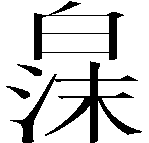
\includegraphics[scale=.5]{muốt.pdf} \kern-.3em}
		\muốt 
\dài}\\[1ex]
xin cho côđơn vào tuổi này\\[1ex]
{\Huge \xin \cho \côđơn \vào \tuổi \này}\\[1ex]
tuổi nào langthang thành phố tóc mây cài\\[1ex]
{\Huge \tuổi \nào \langthang \thànhphố \tóc \mây \cài}\\[1ex]
em xin tuổi nào Còn tuổi nào cho nhau\\[1ex]
{\Huge \em \xin \tuổi \nào \Còn \tuổi \nào \cho \nhau}\\[1ex]
trời xanh trong mắt em sâu\\[1ex]
{\Huge \trời \xanh \trong \mắt \em \sâu}\\[1ex]
mây xuống vây quanh giọt sầu\\[1ex]
{\Huge \mây \xuống \Vây \quanh \giọt \sầu}\\[1ex]
em xin tuổi nào còn tuổi trời hư vô\\[1ex]
{\Huge \em \xin \tuổi \nào \Còn \tuổi \trời \hư \vô}\\[1ex]
bàn tay che dấu lệ  nhòa, ôi buồn\\[1ex]
{\Huge \bàntay \che \dấu \lệ  \nhòa \ôi \buồn}\\[1ex]
tuổi nào ngồi khóc tình đã nghìn thu\\[1ex]
{\Huge \tuổi \nào \ngồi \khóc \tình \đã \nghìn \thu}\\[1ex]
tuổi nào mơ kết mây trong sương mù\\[1ex]
{\Huge \tuổi \nào \mơ \kết \mây \trong \sương \mù}\\[1ex]
xin chân em qua từng phiến ngà\\[1ex]
{\Huge \xin \chân \em \qua \từng \phiến \Ngà}\\[1ex]
xin mây xe thêm màu áo lụa\\[1ex]
{\Huge \xin \mây \Xe \thêm \màu \áo \lụa}\\[1ex]
tuổi nào thôi hết từng tháng năm mong chờ\\[1ex]
{\Huge \tuổi \nào \thôi \hết \từng \tháng \năm \mong \chờ}


\newpage

{\normalsize Đôi mắt người  Sơn Tây}
 
{\Huge \đôi \mắt \người  \sơn \tây}
\bigskip 
 
Em ở thành Sơn chạy giặc về\\[1ex]
{\Huge \em \ở \thành \sơn \chạy \giặc \về}\\[1ex]
Tôi từ chinh chiến cũng ra đi\\[1ex]
{\Huge \tôi \từ \chinh \chiến \cũng \ra \đi}\\[1ex]
Cách biệt bao ngày quê Bất Bạt\\[1ex]
{\Huge \cách \biệt \bao \ngày \quê \bất \bạt}\\[1ex]
Chiều xanh không thấy bóng Ba Vì\\[1ex]
{\Huge \chiều \xanh \không \thấy \bóng \ba \vì}\\[1ex]
Vừng trán em vương trời quê hương\\[1ex]
{\Huge \vừng \trán \em \Vương \trời \quê \hương}\\[1ex]
Mắt em dìu dịu buồn Tây Phương\\[1ex]
{\Huge \mắt \em \dìu \dịu \buồn \tây \phương}\\[1ex]
Tôi nhớ xứ Đoài mây trắng lắm\\[1ex]
{\Huge \tôi \nhớ \xứ \đoài \mây \trắng \lắm}\\[1ex]
Em có bao giờ em nhớ thương?\\[1ex]
{\Huge \em \có \bao \giờ \em \nhớ \Thương}\\[1ex]
Mẹ tôi em có gặp đâu không\\[1ex]
{\Huge \mẹ \tôi \em \có \gặp \đâu \không}\\[1ex]
Bao xác già nua ngập cánh đồng\\[1ex]
{\Huge \bao \XÁc \già \nua \ngập \cánhđồng}\\[1ex]
Tôi nhớ một thằng em bé dại\\[1ex]
{\Huge \tôi \nhớ \một \thằng \em \bé \dại}\\[1ex]
Bao nhiêu rồi xác trẻ trôi sông\\[1ex]
{\Huge \bao \nhiêu \rồi \XÁc \trẻ \trôi \sông}\\[1ex]
Từ độ thu về hoang bóng giặc\\[1ex]
{\Huge \từ \độ \thu \về \hoang \bóng \giặc}\\[1ex]
Điêu tàn thôi lại nối điêu tàn\\[1ex]
{\Huge \điêu \tàn \thôi \lại \nối \điêu \tàn}\\[1ex]
Đất đá ong khô nhiều ngấn lệ\\[1ex]
{\Huge \đất \đá \ong \khô \nhiều \ngấn \lệ}\\[1ex]
Em có bao giờ lệ chứa chan\\[1ex]
{\Huge \em \có \bao \giờ \lệ \chứa \chan}\\[1ex]
Đôi mắt người Sơn Tây\\[1ex]
{\Huge \đôi \mắt \người \sơn \tây}\\[1ex]
U uẩn chiều lưu lạc\\[1ex]
{\Huge \u \uẩn \chiều \lưu \lạc}\\[1ex]
Buồn viễn xứ khôn khuây\\[1ex]
{\Huge \buồn \viễn \xứ \khôn \khuây}\\[1ex]
Tôi gửi niềm thương nhớ\\[1ex]
{\Huge \tôi \gửi \niềm \Thương \nhớ}\\[1ex]
Em mang giùm tôi nhé\\[1ex]
{\Huge \em \MANg \giùm \tôi \nhé}\\[1ex]
Ngày trở lại quê hương\\[1ex]
{\Huge \ngày \trở \lại \quê \hương}\\[1ex]
Khúc hoàn ca rớm lệ\\[1ex]
{\Huge \khúc \hoàn \ca \rớm \lệ}\\[1ex]
Bao giờ trở lại đồng Bương Cấn\\[1ex]
{\Huge \bao \giờ \trở \lại \đồng \bương \cấn}\\[1ex]
Về núi Sài Sơn ngó lúa vàng\\[1ex]
{\Huge \về \núi \sài \sơn \ngó \lúa \VÀng}\\[1ex]
Sông Đáy chậm nguồn qua Phủ Quốc\\[1ex]
{\Huge \sông \đáy \chậm \nguồn \qua \phủ \quốc}\\[1ex]
Sáo diều khuya khoắt thổi đêm trăng\\[1ex]
{\Huge \sáo \diều \khuya \khoắt \thổi \đêm \trăng}\\[1ex]
Bao giờ tôi gặp em lần nữa\\[1ex]
{\Huge \bao \giờ \tôi \gặp \em \lần \nữa}\\[1ex]
Chắc đã thanh bình rộn tiếng ca\\[1ex]
{\Huge \chắc \đã \thanhbình \rộn \tiếng \ca}\\[1ex]
Đã hết sắc mùa chinh chiến cũ\\[1ex]
{\Huge \đã \hết \sắc \mùa \chinh \chiến \cũ}\\[1ex]
Còn có bao giờ em nhớ ta?\\[1ex]
{\Huge \còn \có \bao \giờ \em \nhớ \ta}


\end{document}